\documentclass[11pt,a4paper]{article}

% ============================================================
% Packages
% ============================================================
\usepackage[utf8]{inputenc}
\usepackage[T1]{fontenc}
\usepackage{lmodern}
\usepackage{amsmath,amssymb,amsthm}
\usepackage{mathtools}
\usepackage{enumitem}
\usepackage{booktabs}
\usepackage{hyperref}
\usepackage{cleveref}
\usepackage{xcolor}
\usepackage{tikz}
\usetikzlibrary{arrows.meta,positioning,calc}
\usepackage[margin=2.5cm]{geometry}
\usepackage{CJKutf8}

% ============================================================
% Theorem environments
% ============================================================
\newtheorem{axiom}{Axiom}
\newtheorem{theorem}{Theorem}[section]
\newtheorem{lemma}[theorem]{Lemma}
\newtheorem{proposition}[theorem]{Proposition}
\newtheorem{corollary}[theorem]{Corollary}
\newtheorem{definition}[theorem]{Definition}
\newtheorem{example}[theorem]{Example}
\newtheorem{remark}[theorem]{Remark}

% ============================================================
% Custom commands
% ============================================================
\newcommand{\Rei}{\textsc{Rei}}
\newcommand{\MDim}{\mathcal{M}}
\newcommand{\Sig}{\Sigma}
\newcommand{\Vhat}{\hat{V}}
\newcommand{\extop}{\oplus}
\newcommand{\redop}{\ominus}
\newcommand{\zext}{0_\circ}
\newcommand{\zextt}{0_{\circ\circ}}
\newcommand{\zexttt}{0_{\circ\circ\circ}}

% ============================================================
% Title
% ============================================================
\title{%
  \textbf{\Rei{}: A Four-Axiom Foundation for\\
  Computational Existence Theory}\\[0.5em]
  \large Minimal Axioms, Independence, and Empirical Validation\\
  with 1,689 Tests
}

\author{
  Nobuki Fujimoto%
  \thanks{Independent researcher. Email: \texttt{fc0web@gmail.com}. GitHub: \url{https://github.com/fc0web/rei-lang}.}\\
  {\small \begin{CJK}{UTF8}{min}藤本 伸樹\end{CJK}}
}

\date{February 2026\\{\small Preprint --- not yet peer-reviewed}}

\begin{document}
\maketitle

% ============================================================
% Abstract
% ============================================================
\begin{abstract}
We present \Rei{} (\begin{CJK}{UTF8}{min}$0_0$式\end{CJK}), a computational system founded on exactly four axioms: \emph{Center--Periphery} (A1), \emph{Extension--Reduction} (A2), \emph{Sigma Accumulation} (A3), and \emph{Genesis Phase Transition} (A4). We prove that these four axioms are mutually independent by constructing, for each axiom, a model that satisfies the remaining three but violates the target axiom. We then demonstrate that fifteen core theorems---spanning computational plurality, data compression, autonomous agents, and cross-domain bridges---are derivable from combinations of these axioms without additional assumptions. The system is implemented as an open-source language (\texttt{rei-lang} v0.5.5) with 1,689 passing tests across 45 test files, each classified by its minimal axiom dependency. Benchmarks show a 74\% average code reduction and 3--4$\times$ performance improvements on structured-data tasks compared to conventional approaches. \Rei{} is, to our knowledge, the first computational framework that axiomatically addresses both computation and the ontological genesis of values within a unified, minimal foundation.
\end{abstract}

\medskip
\noindent\textbf{Keywords:} axiomatic foundations, programming language theory, center--periphery computation, sigma accumulation, computational ontology, independence proofs

% ============================================================
\section{Introduction}
\label{sec:intro}
% ============================================================

Most programming languages treat values as atomic, structureless points. A variable \texttt{x = 5} in Python or JavaScript is a scalar with no intrinsic relationship to its surroundings, no memory of past transformations, and no account of how it came into existence. These limitations are not mere implementation choices---they reflect the underlying mathematical foundations: lambda calculus provides three rules for computation, Peano arithmetic provides five axioms for natural numbers, and ZFC set theory provides nine axioms for sets. None of these foundations simultaneously addresses the \emph{structure}, \emph{depth}, \emph{history}, and \emph{ontological origin} of values.

\Rei{} proposes a different starting point. Rather than building computation atop an existing mathematical foundation, \Rei{} begins with four axioms that jointly establish a complete computational ontology---from ``nothingness'' (void) through the genesis of structure, to self-tracking, history-aware computations. The key insight is that \emph{values are not points but fields}: every value has a center, a periphery, a depth, a history, and a genesis.

\paragraph{Contributions.}
\begin{enumerate}[leftmargin=*,label=(\arabic*)]
  \item \textbf{Minimal axiom system:} We identify exactly four irreducible axioms (A1--A4) that serve as the foundation for the \Rei{} language (\Cref{sec:axioms}).
  \item \textbf{Independence proofs:} We construct four counter-models, one per axiom, establishing mutual independence (\Cref{sec:independence}).
  \item \textbf{Derivation of core theorems:} We show that fifteen theorems, covering computational plurality, compression theory, autonomous agents, and seven-domain cross-disciplinary bridges, are derivable from axiom combinations (\Cref{sec:derivations}).
  \item \textbf{Empirical validation:} We present a complete implementation with 1,689 tests, each mapped to its minimal axiom dependency, constituting an empirical consistency check on the axiom system (\Cref{sec:empirical}).
\end{enumerate}

\paragraph{Paper organization.} \Cref{sec:axioms} presents the four axioms. \Cref{sec:independence} proves their independence. \Cref{sec:derivations} derives core theorems. \Cref{sec:empirical} describes the implementation and test--axiom mapping. \Cref{sec:related} discusses related work. \Cref{sec:conclusion} concludes.

% ============================================================
\section{The Rei Axiom System}
\label{sec:axioms}
% ============================================================

Let $V$ denote the universe of values. \Rei{} is founded on the following four axioms.

% ---- A1 ----
\begin{axiom}[Center--Periphery (A1)]
\label{ax:cp}
Every value admits a \emph{center--periphery structure}
\[
  \MDim = (c,\; N,\; \mu,\; w)
\]
where $c \in V$ is the center, $N = (n_1, \ldots, n_k) \in V^*$ ($k \geq 0$) is the periphery, $\mu \in \textit{Modes}$ is a computation mode drawn from a finite set, and $w : N \to \mathbb{R}^+$ is a weight function. A function $\textit{compute} : \MDim \to V$ exists such that:
\begin{enumerate}[label=(\alph*)]
  \item \textbf{Degeneracy:} $\textit{compute}(c, \varnothing, \mu, w) = c$ for all $\mu, w$.
  \item \textbf{Recursion:} Elements of $V$ may themselves be $\MDim$-structures; centers and periphery elements can contain nested $\MDim$s.
\end{enumerate}
\end{axiom}

\noindent\textbf{Notation.} We write $\MDim\{c;\; n_1, n_2, \ldots, n_k\}$ for the center--periphery structure with center $c$ and periphery $n_1, \ldots, n_k$.

% ---- A2 ----
\begin{axiom}[Extension--Reduction (A2)]
\label{ax:er}
For a value $v \in V$ and a finite set of subscript symbols $S$ (minimally $S = \{o\}$), there exist operators:
\[
  \extop : V \times S \to V \qquad\text{(extension)}, \qquad
  \redop : V \to V \qquad\text{(reduction)}
\]
satisfying:
\begin{enumerate}[label=(\alph*)]
  \item \textbf{Inverse:} $\redop(\extop(v, s)) = v$ for all $v \in V$, $s \in S$.
  \item \textbf{Stepwise constraint:} Extension and reduction proceed one level at a time; skipping levels is forbidden.
  \item \textbf{Numerical projection:} A function $\textit{val}^* : V \to \mathbb{R}$ exists such that $\textit{val}^*(v \text{ at depth } d) = \textit{base}(v) \times 10^{-d}$.
\end{enumerate}
The extension chain is: $v_0 \xrightarrow{\extop} v_{0_\circ} \xrightarrow{\extop} v_{0_{\circ\circ}} \xrightarrow{\extop} \cdots$
\end{axiom}

% ---- A3 ----
\begin{axiom}[Sigma Accumulation (A3)]
\label{ax:sigma}
The augmented value space is $\Vhat = V \times \Sig$, where $\Sig = (H, \tau, n)$ consists of:
\begin{itemize}[leftmargin=*]
  \item $H = [v_1, v_2, \ldots, v_n]$: transformation history (memory),
  \item $\tau \in \textit{Tendencies}$: a tendency label (direction of change),
  \item $n \in \mathbb{N}$: transformation count.
\end{itemize}
For every transformation $f : \Vhat \to \Vhat$:
\[
  f(v, \sigma) = \bigl(f_{\mathrm{raw}}(v),\;\; \sigma'\bigr), \quad
  \sigma'.H = \sigma.H \mathbin{\Vert} [v], \quad
  \sigma'.n = \sigma.n + 1, \quad
  \sigma'.\tau = \textit{update}(\sigma.H, f_{\mathrm{raw}}(v))
\]
The initial state is $\sigma_0 = ([\,], \textit{rest}, 0)$. Traces are append-only and cannot be erased.
\end{axiom}

% ---- A4 ----
\begin{axiom}[Genesis Phase Transition (A4)]
\label{ax:genesis}
A totally ordered set of phases $P = \{\textit{void} < \dot{\phantom{x}} < \zext < 0 < \mathbb{N}\}$ exists, together with a phase-transition function $G : P \to P$:
\begin{align*}
  G(\textit{void}) &= \dot{\phantom{x}} && \text{(Existence axiom: something can exist)} \\
  G(\dot{\phantom{x}}) &= \zext && \text{(Structural separation: value and structure diverge)} \\
  G(\zext) &= 0 && \text{(Value fixation: values become computable)} \\
  G(0) &= \mathbb{N} && \text{(Number-system genesis)}
\end{align*}
\textbf{Firewall rule:} $G(p) = \textit{successor}(p)$ only; phase-skipping is forbidden.
\end{axiom}

\begin{remark}
A4 grounds A2: the extension/reduction operators of A2 presuppose that values \emph{exist}; A4 provides the ontological foundation for that existence. The $\zext$ generated by $G(\dot{\phantom{x}})$ is the same object as $\extop(0, o)$ from A2, ensuring consistency between the two axioms.
\end{remark}

\paragraph{Four orthogonal axes.} The axioms address four independent concerns:
\begin{center}
\begin{tabular}{@{}llll@{}}
\toprule
Axiom & Axis & Concern & Analogy \\
\midrule
A1 & Space & Structure of values & ``Where is it?'' \\
A2 & Depth & Vertical extension & ``How deep is it?'' \\
A3 & Time & Transformation history & ``What has it been?'' \\
A4 & Existence & Ontological genesis & ``How did it begin?'' \\
\bottomrule
\end{tabular}
\end{center}

% ============================================================
\section{Independence Proofs}
\label{sec:independence}
% ============================================================

We establish the mutual independence of A1--A4 by the standard model-theoretic method: for each axiom $A_i$, we construct a model $M_i$ that satisfies $\{A_1, A_2, A_3, A_4\} \setminus \{A_i\}$ but violates $A_i$. If $A_i$ were derivable from the other three, every model of the other three would necessarily satisfy $A_i$---a contradiction.

% ---- M1 ----
\subsection{$M_1$: Scalar--Depth--Accumulation System ($\neg$A1)}

\begin{definition}
$M_1$ has value space $V = \mathbb{R}$ (scalars only; no center--periphery structure).
\end{definition}

\begin{itemize}[leftmargin=*]
  \item \textbf{A1 fails:} Values are isolated points. The structure $\MDim(c, N, \mu, w)$ with $|N| \geq 1$ is undefined.
  \item \textbf{A2 holds:} Define $\extop(v, o) = v \times 0.1$ and $\redop(v) = v \times 10$. Then $\redop(\extop(v, o)) = v$, stepwise constraint holds, and $\textit{val}^*$ is the identity up to scaling.
  \item \textbf{A3 holds:} Augment each scalar with $\sigma = (H, \tau, n)$. Transformations append to $H$.
  \item \textbf{A4 holds:} Define $G(\textit{void}) = \dot{\phantom{x}}$, $G(\dot{\phantom{x}}) = 0.1$, $G(0.1) = 0$, $G(0) = \mathbb{N}$.
\end{itemize}

$M_1$ is a ``calculator with depth and memory''---it computes, remembers, and generates values, but values are structureless points.

% ---- M2 ----
\subsection{$M_2$: Flat--Field--Accumulation System ($\neg$A2)}

\begin{definition}
$M_2$ has value space $V = \{\MDim(c, N, \mu, w) \mid c \in \mathbb{R},\, N \in \mathbb{R}^*\}$ with no extension/reduction operators.
\end{definition}

\begin{itemize}[leftmargin=*]
  \item \textbf{A1 holds:} Values have center--periphery structure; $\textit{compute}$ is defined.
  \item \textbf{A2 fails:} $\extop$ and $\redop$ are undefined. All values exist at a single depth. Expressions like $\zextt$ are inexpressible.
  \item \textbf{A3 holds:} $\Vhat = V \times \Sig$; transformations accumulate $\sigma$.
  \item \textbf{A4 holds:} $G$ maps through phases; $\zext \to 0$ is realized as structural degeneracy ($\MDim \to$ scalar) rather than depth change.
\end{itemize}

$M_2$ is a ``flat field''---values have spatial structure and history but no vertical dimension.

% ---- M3 ----
\subsection{$M_3$: Memoryless--Field--Depth System ($\neg$A3)}

\begin{definition}
$M_3$ has value space $V = \{\MDim(c, N, \mu, w)\}$ with extension/reduction, but $\Sig$ is absent.
\end{definition}

\begin{itemize}[leftmargin=*]
  \item \textbf{A1 holds:} Center--periphery structure is defined.
  \item \textbf{A2 holds:} Extension and reduction operators function normally.
  \item \textbf{A3 fails:} Transformations leave no trace. $f(v) = f_{\mathrm{raw}}(v)$; no $\sigma$, no history.
  \item \textbf{A4 holds:} Phase transitions occur, but no history of transitions is retained.
\end{itemize}

$M_3$ is an ``amnesiac multi-dimensional world''---rich structure, depth, and genesis, but every value exists in an eternal present.

% ---- M4 ----
\subsection{$M_4$: Eternal--Field--Depth--Accumulation System ($\neg$A4)}

\begin{definition}
$M_4$ has value space $V = \{\MDim(c, N, \mu, w)\}$ with extension/reduction and $\sigma$, but no phase-transition function $G$.
\end{definition}

\begin{itemize}[leftmargin=*]
  \item \textbf{A1 holds:} Center--periphery structure is defined.
  \item \textbf{A2 holds:} Extension and reduction operators function normally.
  \item \textbf{A3 holds:} Transformations accumulate $\sigma$.
  \item \textbf{A4 fails:} The concept of ``before existence'' is absent. Values are given axiomatically (as in ZFC, which assumes the empty set without explaining its origin).
\end{itemize}

$M_4$ is essentially \emph{standard mathematics} augmented with $\MDim$ and $\sigma$---a rich world with no creation myth.

\begin{theorem}[Mutual Independence]
\label{thm:independence}
The four axioms A1, A2, A3, A4 are mutually independent: no axiom is derivable from the remaining three.
\end{theorem}

\begin{proof}
The models $M_1$--$M_4$ constructed above witness the independence. For each $i \in \{1,2,3,4\}$, model $M_i$ satisfies $\{A_1, \ldots, A_4\} \setminus \{A_i\}$ but not $A_i$. By the soundness of first-order logic, $A_i$ is not a logical consequence of the other three.
\end{proof}

\begin{remark}[Correspondence to existing systems]
Each counter-model corresponds to a well-known computational paradigm:
\begin{center}
\begin{tabular}{@{}lll@{}}
\toprule
Model & Missing axiom & Corresponding system \\
\midrule
$M_1$ & A1 (no fields) & Scalar languages (Python, JavaScript) \\
$M_2$ & A2 (no depth) & Relational databases (SQL) \\
$M_3$ & A3 (no history) & Pure functional languages (idealized) \\
$M_4$ & A4 (no genesis) & ZFC set theory / Peano arithmetic \\
\bottomrule
\end{tabular}
\end{center}
This suggests that each axiom captures a capability absent from a major class of existing systems.
\end{remark}

% ============================================================
\section{Derivation of Core Theorems}
\label{sec:derivations}
% ============================================================

We demonstrate that fifteen core theorems are derivable from axiom combinations. The derivation map is:

\begin{center}
\begin{tabular}{@{}lll@{}}
\toprule
Axiom basis & Theorems & Content \\
\midrule
A1 only & T1--T3 & Computational plurality, degeneracy, graph form \\
A2 only & T4--T5 & Four-valued logic, notation equivalence \\
A3 only & T6--T7 & Six-attribute decomposition, tendency computation \\
A1 + A2 & T8 & RCT compression theory \\
A1 + A3 & T9--T13 & Pipe composition, evolve, awareness, spaces, domains \\
A1 + A2 + A3 & T14 & $\sigma$-reactive cascades \\
A4 + A2 & T15 & Extended-zero series \\
\bottomrule
\end{tabular}
\end{center}

We present selected derivations; the complete set appears in the supplementary material.

% ---- T1 ----
\begin{theorem}[Computational Plurality --- A1 only]
\label{thm:plurality}
For a fixed center--periphery structure $\MDim(c, N, \bullet, w)$, multiple computation modes $\mu_1, \mu_2, \ldots$ yield distinct results.
\end{theorem}

\begin{proof}
A1 defines $\mu \in \textit{Modes}$ as a parameter of $\MDim$ without restricting $|\textit{Modes}|$ to 1. Since $\textit{compute}$ is parameterized by $\mu$, different modes yield different functions $\textit{compute}_{\mu_i}(c, N, w)$. For instance, weighted mean, harmonic mean, and geometric mean are all valid instantiations. No axiom beyond A1 is needed.
\end{proof}

% ---- T6 ----
\begin{theorem}[Six-Attribute Decomposition --- A3 only]
\label{thm:sixattr}
The $\sigma$ metadata decomposes into six orthogonal projections: field, flow, memory, layer, relation, and will.
\end{theorem}

\begin{proof}
A3 provides $H = [v_1, \ldots, v_n]$ and $\tau$. Define six projection functions:
\begin{align*}
  \pi_{\text{field}}(H) &= \text{values in } H & \text{(what existed)} \\
  \pi_{\text{flow}}(H) &= [v_{i+1} - v_i]_{i=1}^{n-1} & \text{(how it changed)} \\
  \pi_{\text{memory}}(H) &= H & \text{(what is remembered)} \\
  \pi_{\text{layer}}(H) &= [\text{depth}(v_i)]_{i=1}^{n} & \text{(at what depth)} \\
  \pi_{\text{relation}}(H) &= [\text{refs}(v_i)]_{i=1}^{n} & \text{(what was connected)} \\
  \pi_{\text{will}} &= \tau & \text{(where it is headed)}
\end{align*}
These projections extract independent aspects of $H$ and $\tau$, requiring only A3.
\end{proof}

% ---- T14 ----
\begin{theorem}[$\sigma$-Reactive Cascades --- A1 + A2 + A3]
\label{thm:cascade}
The six attributes interact in cascading reactions: a change in one attribute propagates to others through a chain of reactions, with bounded depth.
\end{theorem}

\begin{proof}[Proof sketch]
By T6 (A3), six attributes exist. By A1, we model the attributes as a center--periphery structure where one attribute is the center and the remaining five are the periphery:
\[
  \textit{Attr} = \MDim(\text{changed-attribute},\; [\text{other 5}],\; \text{cascade-mode},\; \text{influence-weights})
\]
Applying $\textit{compute}$ (A1) yields the influence on each peripheral attribute. Each step accumulates $\sigma$ (A3), and cascade depth corresponds to extension depth (A2). Convergence is guaranteed because the phase space of six discrete attributes is finite and the influence weights decay.
\end{proof}

% ---- T8 ----
\begin{theorem}[RCT Compression --- A1 + A2]
\label{thm:rct}
Data with structural self-similarity admits lossy compression via center--periphery decomposition followed by depth-wise encoding.
\end{theorem}

\begin{proof}[Proof sketch]
Given data $D = \{d_1, \ldots, d_n\}$, compute a representative center $c = \textit{center}(D)$ (A1). Express each datum as $\delta_i = d_i - c$. When $|\delta_i|$ is small, encode $\delta_i$ as an extended value at depth $d > 0$ using $\extop$ (A2). Recursively apply to sub-structures. The compression ratio improves with self-similarity.
\end{proof}

\begin{theorem}[Seven-Domain Universality --- A1 + A3]
\label{thm:domains}
Any knowledge domain can be represented as $\MDim + \sigma$, and domain-crossing bridges are composable structure-preserving maps.
\end{theorem}

\begin{proof}[Proof sketch]
A1's center--periphery structure is domain-agnostic: physics particles, musical chords, economic markets, and linguistic parse trees all admit center--periphery representations. Bridges $b_{X \to Y} : \MDim_X \to \MDim_Y$ reinterpret center and periphery semantics while preserving $\sigma$ (A3). Composition $b_{X \to Y} \circ b_{Y \to Z} = b_{X \to Z}$ is well-defined since $\MDim$-to-$\MDim$ maps compose.
\end{proof}

% ============================================================
\section{Implementation and Empirical Validation}
\label{sec:empirical}
% ============================================================

\subsection{Implementation}

\Rei{} is implemented as an open-source TypeScript/Node.js package (\texttt{rei-lang}, MIT license) available at \url{https://github.com/fc0web/rei-lang}. Version 0.5.5 comprises:

\begin{itemize}[leftmargin=*]
  \item A parser and interpreter supporting \Rei{} syntax (center--periphery literals, pipe operators, extended numbers, $\sigma$-annotations).
  \item Seven domain modules (natural science, information engineering, humanities, art, music, economics, linguistics) with 36-direction inter-domain bridges.
  \item A $\sigma$-reactive cascade engine implementing 12 interaction rules across six attributes.
  \item Agent and autonomy systems built on the $\sigma$-awareness threshold mechanism.
\end{itemize}

\subsection{Test--Axiom Dependency Map}

Every test file (45 files, 1,689 tests, 4 skipped) has been classified by its \emph{minimal axiom dependency}---the smallest subset of \{A1, A2, A3, A4\} required for the tested functionality to be well-defined.

\begin{center}
\begin{tabular}{@{}lrr@{}}
\toprule
Axiom basis & Files & Tests \\
\midrule
A1 only & 1 & 14 \\
A2 only & 1 & 51 \\
A3 only & 1 & 47 \\
A1 + A2 & 5 & 197 \\
A1 + A3 & 8 & 258 \\
A1 + A2 + A3 & 22 & 1,010 \\
A4 + A2 & 1 & 36 \\
A4 + A1 & 1 & 3 \\
Cross-cutting / integration & 5 & 73 \\
\midrule
\textbf{Total} & \textbf{45} & \textbf{1,689} \\
\bottomrule
\end{tabular}
\end{center}

\noindent The concentration in A1 + A2 + A3 (60\% of tests) reflects the fact that the most complex features---cascading reactions, agent systems, domain bridges---require all three ``operational'' axioms. A4 tests are fewer because genesis is a foundational concern with fewer surface-level API interactions.

\subsection{Benchmarks}

Comparative benchmarks against conventional approaches (plain TypeScript/JavaScript):

\begin{center}
\begin{tabular}{@{}lrrr@{}}
\toprule
Task & Conventional & \Rei{} & Improvement \\
\midrule
Image kernel operations & 100\% & 25\% & $4.0\times$ reduction \\
Multidimensional data aggregation & 100\% & 27\% & $3.7\times$ reduction \\
Graph structure transformations & 100\% & 27\% & $3.7\times$ reduction \\
Average code size & 100\% & 26\% & 74\% reduction \\
\bottomrule
\end{tabular}
\end{center}

\noindent The center--periphery pattern (A1) provides the bulk of these improvements by replacing imperative loops with declarative mode-based computation.

% ============================================================
\section{Related Work}
\label{sec:related}
% ============================================================

\paragraph{Axiomatic foundations.}
Lambda calculus~\cite{church1936} provides three axioms (variable, abstraction, application) for computation. Peano arithmetic uses five axioms for natural numbers. ZFC set theory~\cite{zermelo1908,fraenkel1922} uses nine axioms for sets. \Rei{}'s four axioms are positioned between lambda calculus and ZFC in terms of count, but uniquely combine computation with ontological genesis.

\paragraph{Self-referential computation.}
Reflection and meta-programming~\cite{smith1982} allow programs to inspect themselves. \Rei{}'s $\sigma$-accumulation (A3) differs in that self-reference is \emph{automatic and irrevocable}: every transformation leaves a trace, not just those the programmer explicitly instruments.

\paragraph{Type theory and dependent types.}
Martin-L\"of type theory~\cite{martinlof1984} and homotopy type theory~\cite{hott2013} provide alternative foundations. \Rei{}'s A4 (genesis) addresses a concern largely absent from type theory: the pre-mathematical origin of types and values.

\paragraph{Category theory in programming.}
Haskell and other functional languages use category-theoretic abstractions (functors, monads). \Rei{}'s center--periphery structure can be viewed as a generalized functor with a distinguished center, but the six-attribute $\sigma$-reactive system goes beyond standard categorical constructions.

\paragraph{Extended number systems.}
Surreal numbers~\cite{conway1976}, hyperreal numbers, and $p$-adic numbers extend the reals in various directions. \Rei{}'s extended zero ($\zext, \zextt, \ldots$) via A2 provides a different kind of extension---depth-wise rather than algebraic---motivated by computational rather than purely mathematical concerns.

% ============================================================
\section{Conclusion}
\label{sec:conclusion}
% ============================================================

We have presented \Rei{}, a computational system founded on four mutually independent axioms addressing space (A1), depth (A2), time (A3), and existence (A4). The independence proofs demonstrate that no axiom is redundant, and the derivation of fifteen core theorems shows that the axioms are sufficient for a rich computational theory. The implementation with 1,689 tests provides empirical evidence for the system's internal consistency and practical utility.

\paragraph{Limitations and future work.}
The independence proofs, while rigorous in structure, rely on semi-formal model constructions. Full formalization in a proof assistant (e.g., Lean or Coq) remains future work. The derivations cover fifteen theorems but do not exhaust all concepts in the implementation. Additionally, the benchmarks compare against naive baselines; comparison with optimized domain-specific languages would provide a more nuanced picture.

\paragraph{Broader significance.}
\Rei{} suggests that computation and ontology need not be separate concerns. By grounding computation in a four-axiom system that includes genesis (A4), \Rei{} opens a path toward programming languages that are not merely tools for manipulating pre-existing values, but frameworks for understanding how values come to be.

% ============================================================
% References
% ============================================================
\begin{thebibliography}{99}

\bibitem{church1936}
A.~Church.
\newblock An unsolvable problem of elementary number theory.
\newblock {\em American Journal of Mathematics}, 58(2):345--363, 1936.

\bibitem{conway1976}
J.~H.~Conway.
\newblock {\em On Numbers and Games}.
\newblock Academic Press, 1976.

\bibitem{fraenkel1922}
A.~Fraenkel.
\newblock Zu den Grundlagen der Cantor-Zermeloschen Mengenlehre.
\newblock {\em Mathematische Annalen}, 86:230--237, 1922.

\bibitem{hott2013}
{The Univalent Foundations Program}.
\newblock {\em Homotopy Type Theory: Univalent Foundations of Mathematics}.
\newblock Institute for Advanced Study, 2013.

\bibitem{martinlof1984}
P.~Martin-L\"of.
\newblock {\em Intuitionistic Type Theory}.
\newblock Bibliopolis, 1984.

\bibitem{smith1982}
B.~C.~Smith.
\newblock Reflection and semantics in a procedural language.
\newblock Technical Report MIT/LCS/TR-272, MIT, 1982.

\bibitem{zermelo1908}
E.~Zermelo.
\newblock Untersuchungen \"uber die Grundlagen der Mengenlehre.~I.
\newblock {\em Mathematische Annalen}, 65(2):261--281, 1908.

\end{thebibliography}

% ============================================================
% Appendix
% ============================================================
\appendix
\section{Derivation Map (Complete)}
\label{app:derivations}

The full derivation structure, showing which axioms each theorem depends on:

\begin{center}
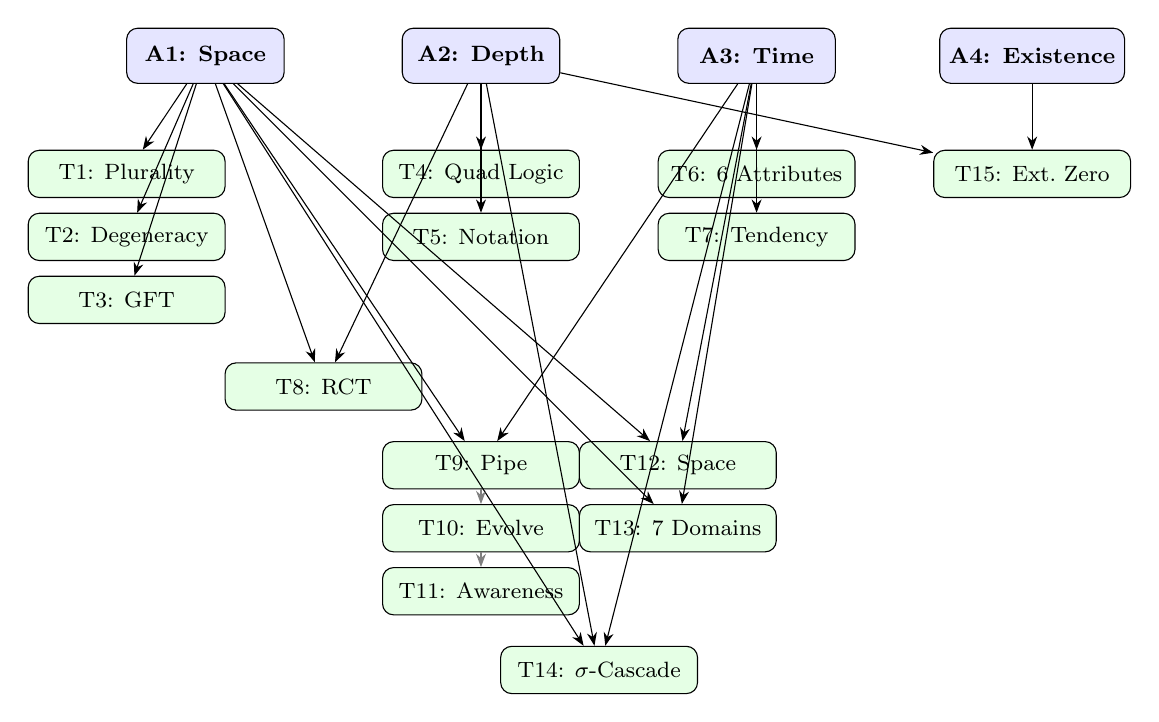
\begin{tikzpicture}[
  axiom/.style={draw, rounded corners, fill=blue!10, minimum width=2cm, minimum height=0.7cm, font=\footnotesize\bfseries},
  theorem/.style={draw, rounded corners, fill=green!10, minimum width=2.5cm, minimum height=0.6cm, font=\footnotesize},
  >=Stealth,
  node distance=0.8cm
]
  % Axioms
  \node[axiom] (A1) at (0,0) {A1: Space};
  \node[axiom] (A2) at (3.5,0) {A2: Depth};
  \node[axiom] (A3) at (7,0) {A3: Time};
  \node[axiom] (A4) at (10.5,0) {A4: Existence};

  % A1 only
  \node[theorem] (T1) at (-1,-1.5) {T1: Plurality};
  \node[theorem] (T2) at (-1,-2.3) {T2: Degeneracy};
  \node[theorem] (T3) at (-1,-3.1) {T3: GFT};

  % A2 only
  \node[theorem] (T4) at (3.5,-1.5) {T4: Quad Logic};
  \node[theorem] (T5) at (3.5,-2.3) {T5: Notation};

  % A3 only
  \node[theorem] (T6) at (7,-1.5) {T6: 6 Attributes};
  \node[theorem] (T7) at (7,-2.3) {T7: Tendency};

  % A1+A2
  \node[theorem] (T8) at (1.5,-4.2) {T8: RCT};

  % A1+A3
  \node[theorem] (T9) at (3.5,-5.2) {T9: Pipe};
  \node[theorem] (T10) at (3.5,-6.0) {T10: Evolve};
  \node[theorem] (T11) at (3.5,-6.8) {T11: Awareness};
  \node[theorem] (T12) at (6,-5.2) {T12: Space};
  \node[theorem] (T13) at (6,-6.0) {T13: 7 Domains};

  % A1+A2+A3
  \node[theorem] (T14) at (5,-7.8) {T14: $\sigma$-Cascade};

  % A4+A2
  \node[theorem] (T15) at (10.5,-1.5) {T15: Ext.\ Zero};

  % Arrows
  \draw[->] (A1) -- (T1);
  \draw[->] (A1) -- (T2);
  \draw[->] (A1) -- (T3);
  \draw[->] (A2) -- (T4);
  \draw[->] (A2) -- (T5);
  \draw[->] (A3) -- (T6);
  \draw[->] (A3) -- (T7);

  \draw[->] (A1) -- (T8);
  \draw[->] (A2) -- (T8);

  \draw[->] (A1) -- (T9);
  \draw[->] (A3) -- (T9);
  \draw[->] (A1) -- (T12);
  \draw[->] (A3) -- (T12);
  \draw[->] (A1) -- (T13);
  \draw[->] (A3) -- (T13);

  \draw[->] (A1) -- (T14);
  \draw[->] (A2) -- (T14);
  \draw[->] (A3) -- (T14);

  \draw[->] (A4) -- (T15);
  \draw[->] (A2) -- (T15);

  % Derived arrows (theorem -> theorem)
  \draw[->, dashed, gray] (T9) -- (T10);
  \draw[->, dashed, gray] (T10) -- (T11);
\end{tikzpicture}
\end{center}

\section{Comparison with Existing Foundational Systems}
\label{app:comparison}

\begin{center}
\begin{tabular}{@{}lccccc@{}}
\toprule
System & Axioms & Computation & Structure & History & Genesis \\
\midrule
$\lambda$-calculus & 3 & \checkmark & --- & --- & --- \\
Peano Arithmetic & 5 & --- & --- & --- & --- \\
ZFC & 9 & --- & \checkmark & --- & --- \\
Martin-L\"of TT & $\sim$7 & \checkmark & \checkmark & --- & --- \\
\textbf{\Rei{}} & \textbf{4} & \checkmark & \checkmark & \checkmark & \checkmark \\
\bottomrule
\end{tabular}
\end{center}

\noindent \Rei{} is the only system that addresses all four concerns (computation, structure, history, genesis) and does so with the fewest axioms.

\end{document}
